\paragraph{Definition:} Causal reasoning refers to the ability to infer, analyze, understand, and explain the causal relationships between events and actions. 
Tasks in this domain can be classified into the following parts:

\begin{enumerate}
    \item \textbf{Causal discovery}:  Identifying causal relationships between two or more events. 
    This typically answers questions like: Is event A the cause of event B?

    \item \textbf{Effect inference}:   Once the causes of an outcome are known, it is important to understand how much those causes contribute to the outcome.
    In other words, one seeks to estimate the magnitude of the cause’s impact on the current result.\
    
    \item \textbf{Attribution}: The goal of this task is to identify which cause is the main driver behind a specific change.
    \item \textbf{Judgment}: This is an extension of Attribution, where rewards or blame are assigned to actions based on other causal relationships
    In other words, it makes decisions based on causal relationships. 
\end{enumerate}

\begin{figure}
    \centering
    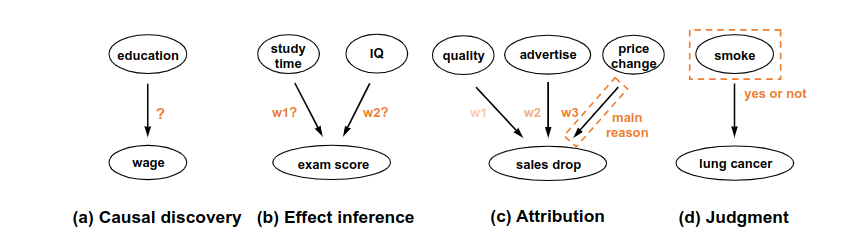
\includegraphics[width=0.9\textwidth]{Figs/causal_graph.png}
    \caption{Causal graph describe the four tasks of Causal Reasoning}
    \label{fig:causal_graph}
\end{figure}


To represent these relationships, causal graphs (causal networks) are used, which are graphs depicting the causal relationships between variables or events. 
In such graphs, variables or events are represented by nodes, and the causal relationships between them are represented by directed arrows. 
Figure \ref{fig:causal_graph} uses a causal graph to describe the four tasks mentioned above


\subsubsection{Counterfactual Reasoning}

Counterfactual \cite{li2023counterfactual} is introduced as a method to assess the reasoning and understanding abilities of large language models in hypothetical scenarios. 
In this context, counterfactuals are defined as things that are false in the real world but true in a hypothesis
Since most large language models are trained on human knowledge or real-world knowledge, having the model reason based on hypothetical knowledge 
(which it may not have learned or known) can expand and evaluate its reasoning ability, forcing it to make unusual conclusions or predictions


\paragraph{Formula:} Let x $\in$ X be the input, where X represents knowledge $w$ in the worlds W, to produce an output $y \in Y$. This defines a function $f$ that perfomrs
a mapping: X $\rightarrow$ Y. The counterfactual reasoning is defined as the function $f_{cf}$: X $\times$ W $\rightarrow$ Y. Assuming that $h$ approximates functions $f_w$, where w 
can be real world or counterfactual world, a large language model implementing $f_w$ can be described as follows: 

\[
h(f, w, x) = argmax_{y \in Y} P_{LM}(y' | prompt_f(f, x), prompt_w(w))
\]

where $prompt_f$ and $prompt_w$ are the prompts for the function $f$. 


The study \cite{wu2023reasoning} employs counterfactual reasoning to evaluate the abstract reasoning capabilities of large language models (LLMs). 
The paper proposes a framework consisting of 11 hypothetical tasks designed to assess the reasoning abilities of LLMs. 
The performance of models such as GPT-4, Claude, and PaLM-2 is compared across tasks in both default worlds and counterfactual worlds.
The findings indicate that current models can handle abstract tasks to a certain extent. However, their capabilities are heavily dependent on narrow, context-specific settings, 
highlighting the limitations in generalizing abstract reasoning across diverse context. 

Additionally, the study \cite{li2023counterfactual} investigates how pretrained language models (PLMs) handle counterfactual conditions. 
The primary goal of the research is to assess whether PLMs can distinguish between hypothetical situations and real-world scenarios
The study concludes that when faced with counterfactual situations, PLMs often generate text that contradicts established real-world knowledge
. Furthermore, PLMs tend to prioritize closer contextual information over more general knowledge when reasoning in hypothetical scenarios. This indicates that language models are not only influenced 
y the world knowledge they have learned but are also affected by the linguistic structure and the specific context of the scenarios presented to them.

\subsubsection{Enhance the Causal Reasoning Capabilities of LLMs}
From the studies discussed above, large language models (LLMs) exhibit significant limitations in causal reasoning, particularly in tasks that demand deep understanding and analysis of cause-effect relationships.
To address these issues, the study \cite{xiong2024improving} summarizes several methods to improve the reasoning abilities of LLMs. These methods are categorized into two main approaches (Figure \ref{fig:causal_method}):

\begin{figure}
    \centering
    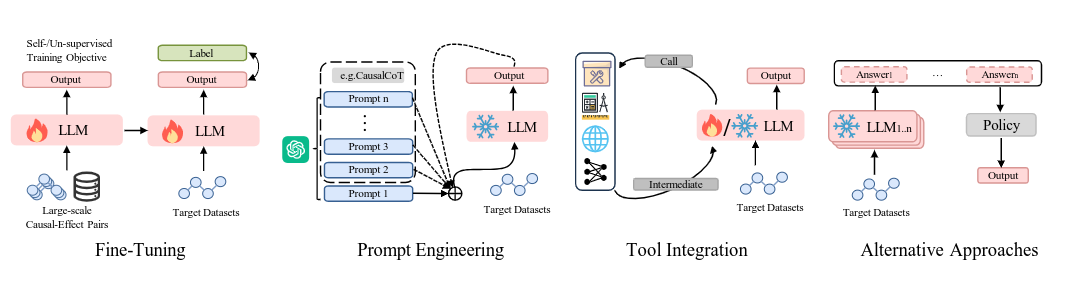
\includegraphics[width=0.9\textwidth]{Figs/causal_method.png}
    \caption{Overview of methods for LLMs as causal reasoning engine}
    \label{fig:causal_method}
\end{figure}


\begin{enumerate}
    \item \textbf{Using LLMs as Tools for Causal Reasoning}: This approach involves leveraging LLMs to infer causal rules through techniques such as fine-tuning, prompting, or other task-specific adjustments.
    \item \textbf{Supporting Traditional Causal Inference Methods with LLMs}: In this approach, LLMs are utilized to assist in traditional causal reasoning methods by extracting causal information from data or generating synthetic causal datasets.
\end{enumerate}

\paragraph{Fine-tuning} This method leverages the prior knowledge learned by pretrained models and adapts it to perform new tasks, significantly reducing the training time compared to training a model from scratch.
Research \cite{li2021causalbert} applied self-supervised learning combined with fine-tuning techniques to enable pretrained models to learn causal knowledge. Additionally, \cite{zheng2023preserving} introduced the Causal Effect Tuning method, which facilitates 
learning new knowledge based on target data while preserving the pretrained model's prior knowledge.
However, this approach has a major requirement: datasets must have a clear structure and labeling for the model to fine-tune effectively. Unfortunately, most datasets available today are unstructured and collected from the web, which limits the effectiveness of this method.
To address this, \cite{jiang2023large} collected datasets containing causal questions and structured interpreted intents with a specific format to support fine-tuning. Furthermore, \cite{chen2024unified} combined Structural Causal Models (SCM) with instruction-tuning techniques to develop
Structural Instruction Tuning, which learns causal representations specific to each task by simulating causal factors and relationships.
This method provides a promising way to enhance the causal reasoning capabilities of LLMs, although it remains dependent on the availability of high-quality, structured datasets

\paragraph{Prompting} In addition to fine-tuning, large language models (LLMs), trained on vast datasets, can perform certain tasks directly through prompting without prior task-specific training—a technique known as in-context learning. This approach is advantageous as it requires fewer resources, is simpler to implement, and can achieve results comparable to fine-tuning.
However, causal reasoning (CR) often involves multiple steps and complex relationships, requiring deeper understanding and reasoning capabilities from the model. To address these challenges, researchers have introduced prompting-based methods to enhance the causal reasoning abilities of LLMs:

\begin{enumerate}
    \item \textbf{Causal Chain-of-Thought (CausalCoT)}: Built upon the Chain-of-Thought (CoT) methodology, CausalCoT \cite{jin2023cladder} is designed to guide models in step-by-step reasoning through complex causal relationships, ensuring clarity and accuracy in their outputs.
    \item \textbf{Causal Contextualized Learning (CausalCL)} \cite{wang2023contextualized}: Combines code-like prompting with CoT to support multistep event reasoning. This approach improves the model's ability to analyze interconnected causal events and enhances reasoning precision.
    \item \textbf{Multi-modal Causal Reasoning (MCR)} \cite{zang2023discovering}: Introduces causal reasoning using multimodal inputs, enabling the model to reason not only from text but also by analyzing images. This expands the scope of causal reasoning to visual contexts and real-world scenarios.
    \item \textbf{Counterfactual Prompting Learning (CPL)} \cite{he2022cpl}: Leverages counterfactual scenarios, allowing the model to explore and reason through hypothetical, non-realistic assumptions. This method enhances the model's causal understanding by encouraging it to think beyond established knowledge.
\end{enumerate}

\paragraph{External tools} In addition to improving the core capabilities of LLMs, another approach is to utilize external tools such as knowledge bases, search systems, or specialized reasoning computation systems. This allows LLMs to continuously update knowledge without the need of fine-tuning to incorporate new information
and to leverage external computation systems (including other LLMs) to handle more complex reasoning tasks.
For instance, research \cite{lu2022neuro} introduces a causal framework for procedural planning using a knowledge base like ConceptNet. It analyzes the semantics of text into entity sets and retrieves relevant sub-graphs to improve planning. 
Furthermore, research \cite{pawlowski2023answering} compares context augmentation and tool-augmentation methods. Context augmentation uses LLMs to perform auxiliary tasks outside the system, while tool augmentation employs Python scripts to process results from the system. 
The study demonstrates that models using tool augmentation make fewer errors compared to context augmentation.
However, this approach also faces several limitations, primarily its reliance on the quality of external resources and the need for synchronization between the model and the tools


\paragraph{Enhancing Traditional CR Methods} Not only serving as a tool with causal reasoning capabilities, LLMs can also support traditional causal analysis methods in the following ways:

\begin{figure}
    \centering
    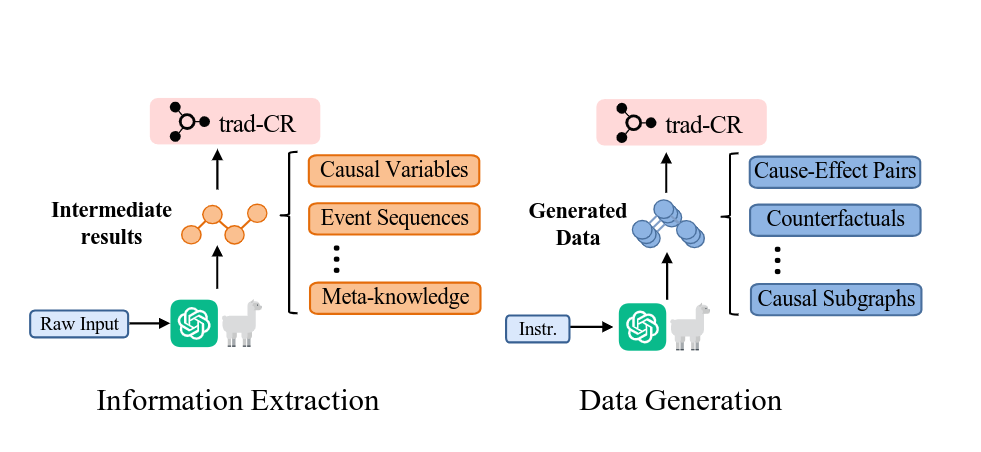
\includegraphics[width=0.9\textwidth]{Figs/causal_trandition_imprv.png}
    \caption{Overview of methods for using LLMs to enhance traditional approache}
    \label{fig:causal_tradition}
\end{figure}

\begin{enumerate}
    \item \textbf{Causal Information Extraction}: Extracting causal event chains and variables from unstructured text or identifying causal relationships in real-world scenarios.
    \item \textbf{Causality Data Generation and Augmentatio}: Generating cause-effect pairs, counterfactuals, and causal subgraphs, while also proposing hypotheses about causal relationships within observed data
\end{enumerate}